\section{Introduction}
This paper is about an academic project born to be an efficient solution for the CINI\footnote{Consorzio Interuniversitario Nazionale per l'Informatica} 2017 Challenge on smart cities illumination systems. In particular, the goal was to prototype and test a solution which was capable of (near) real-time data stream processing for monitoring records from streetlamps, lumen sensors co-located with the streetlamp itself and from traffic data produced by third-party APIs. We will explore this solution for the following use case: in a smart city context it is necessary to guarantee the maximum efficiency from lamps consumption while providing an optimal illumination within safety limits for pedestrians and drivers and according to local traffic intensity. To achieve that, it is necessary to project a grid of smart lamps capable of tuning their light level according to the right amount of energy necessary to provide city aware, safe and green consumption levels. This grid must be powered and managed via a reliable, highly available, processing-capable control system. Introducing Project Ember.

\section{Frameworks and Tools}
Managing a data stream processing system was a challenge that we wanted to take, being something never experienced before. So, based upon our knowledge, we structured our environment using at first a publish/subscribe architecture with the street lamps, lumen and traffic sensors as publishers and the stream processing framework as subscriber. Talking about the Publish/Subscribe frameworks,  different offers are available over the open source community. RabbitMQ\footnote{RabbitMQ documentation: https://www.rabbitmq.com/getstarted.html} and Apache Kafka\footnote{Apache Kafka documentation: https://kafka.apache.org/documentation/} were our favorite choices, but the exploration of the documentation of that which would be our Data Stream Processing framework made possible the final decision. The Apache Software Foundation makes available different alternatives, each one a refined version of the previous: Apache Storm\footnote{Apache Storm official page: http://storm.apache.org/} is one of the most used data stream processing framework on the market and one of the most supported as well; Apache Spark\footnote{Apache Spark official page: http://spark.apache.org/} is a refined version of Storm even though it is limited to fewer programming languages (Java, Scala and Python); Apache Flink\footnote{Apache Flink official page: https://flink.apache.org/} is the most recent project among the three and the most advanced. Flink gives the programmer the possibility to define just the topology of the operators, how they are linked, or how to set the windows timing (based upon the event or upon the processing inside the system). Flink thinks about the rest: multithreading, synchronization, parallelism, availability, cluster management are our interest no more, Flink takes care of them for us. We choosed the latest stable release of Apache Flink, 1.2, which comes with a well written documentation as well as multiple connectors for the most popular publish/subscribe or persistency platform. Flink calls a Source that component that produce data and Sink the one that takes the processed data in order to persistence them or to route them. Apache Kafka works seamlessly with Flink thanks to the included connector plugins giving the possibility to simply personalize the connection according to our preferences: Kafka is our Source. Talking about Sink, Flink supports many platforms and Kafka can be one of them, but in order to persist and manage our data we wanted to use a modern platform capable of organizing data for (near) real-time purposes, properties not so common for databases with RDBMS engines. A NoSQL approach was mandatory to us, so we analyzed different products: Elasticsearch\footnote{Elasticsearch official page: https://www.elastic.co/products/elasticsearch} and Apache Cassandra\footnote{Apache Cassandra official page: http://cassandra.apache.org/}. Elasticsearch is fully supported (not its last version) by Flink 1.2 and is flexible, easy-to-deploy database with RESTful APIs. It makes possible every type of query, even geographical ones, in a fast and simple way. Elasticsearch is part of the Elastic Stack built by Elastic.co which makes available another useful tool for visualizing data stored in Elasticsearch linking and visualizing them according to our preferences, Kibana\footnote{Kibana official page: https://www.elastic.co/products/kibana}. That's why Apache Cassandra was not chosen at last although it seemed obvious for us at first, being part of the Apache Software Foundation and respecting the configuration formats of the other components of the system.
The choice of the framework that would realize our persistence level has been influenced by the search of a simple and elegant visualization platform for our data. Elasticsearch has Kibana, but we really wanted to use Grafana\footnote{Grafana official page: https://grafana.com/} at first. Grafana offers different connector for the most famous persistence platform, Elasticsearch included. We analyzed InfluxDB\footnote{InfluxDB official page: https://www.influxdata.com/}: fully supported by Grafana but it would require a great amount of effort for using it with Flink which doesn't have an official connector. While Grafana can connect to Elasticsearch, its deploying and configuration looked complicated to configure in order to obtain even an adequate visualization and time wasn't our side.Kibana instead was incredibly easy to deploy, having only to specify the Elasticsearch database you want to use, understanding the data format inside the database. 
Java is the programming language that links all these components together being used by Flink as well as Scala, such as Elasticsearch APIs. 
Once defined our components, let’s see how they relate to each other: Lamps and Flink produce a lot of data in streams that Kafka organizes in topics. A topic for lamps, lumens and traffic are created being specific. A system such as this can be very efficient but let’s think about the next step. Being a Smart Lamp Grid the system has to emit orders directed to a single lamp among thousands. Kafka can manage runtime topics creation but a topic for a single lamp is meaningless and inefficient and require the data stream processing system to know the right position of the lamp among the network. So we decided to build a Control Unit using Flask and Redis. Flask\footnote{Flask official page: http://flask.pocoo.org/} is a micro-framework for Web Server built in Python and Redis\footnote{Redis official page: https://redis.io/} is one of the most famous in-memory data store. We will analyze the Control Unit later, let's see why Flask and Redis. We needed a web server component capable of directing lamps data to Kafka and directive from Flink-Kafka to lamps. Flask is a framework we used a lot for realizing web servers. Flask allows us to define entrypoint with a single line of code and RESTful APIs in seconds. Flask its also very efficient being multithreaded and easy to deploy thanks to Python. Redis instead its a really fast data store as a database, cache and message broker. Redis serves us as a cache, maintaing a good amount of data per Control Unit but allowing us to interact with it with very simple APIs and to deploy it being Docker friendly.

\section{Architecture overview}
In this section we will cover how the system communicates between each of its components and modules and the assumptions we made to prototype and test the architecture. In \hyperref[fig:ember_architecture]{figure 1} a high-level architecture overview is provided. Before proceeding, we want to focus on the output from the real-time\footnote{We will define the system as "real-time" in this paper even if is not validated for such a control system, but it is capable of near real-time data streams processing} control system: it is produced into the MOM\footnote{Messages Oriented Middleware} and consumed by control units (how will be discussed later), closing a feedback loop. This behavior and the capabilities to maintain high-availability across the clusters make the system itself near to the features of an autonomic system.
\begin{figure}
\begin{center}
	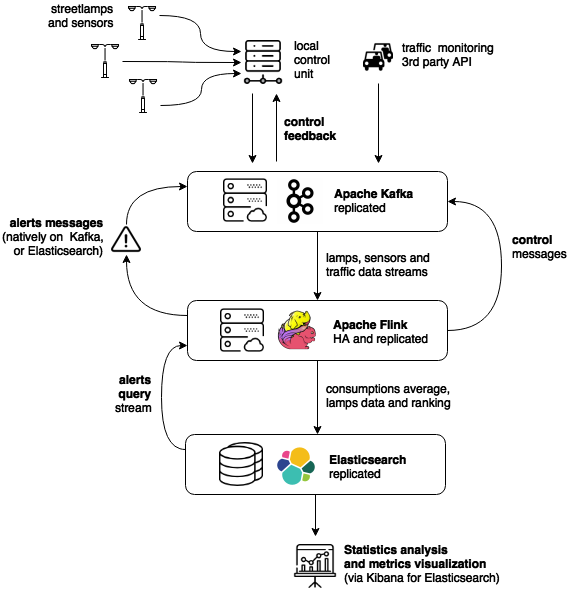
\includegraphics[scale=0.35]{img/ember_architecture}
	\caption{Project Ember architecture overview}
	\label{fig:ember_architecture}
\end{center}
	
\end{figure}


\subsection{Sensors network}
First of all let us consider how the sensors network [...]. According to project specifications the street lamps sends to the system a JSON formatted string containing all the information their microcontrollers collect. Those data are sent every 10 seconds. A lumen sensor is placed on the lamp and it sent data with same rate as well giving us information about the daylight luminosity level and the id of the lamps he is placed upon.

\subsection{Control Unit}
The Control Unit gives us the possibility to create a new indirection level that is placed among the lamps and Flink. The lamps talks to the Control Unit which maintains a mapping between the lamps ids and their IP addresses inside the local city network. The lamps has to be registered to the right control unit in order to submit their data inside the system which increase the security level of our system (such operation need to be done by the operator that place the lamp). The Control Unit validates the lamps and sends their data to Kafka lamp topic. One the response will be made available the Control Unit takes care to be registered to the topic of its own, so it can take the responses and understand to which lamp direct them. Kafka makes possible all of this, making our system totally plug and play. Flink on the other hand is registered on the main three topics: lamps, lumen, traffic. Flink processes them calculating the right lumen value a lamp should have, a rank of the most-probable-to-fail lamps and consumption means per streets and/or per ids. Some data needs to be sent the right lamp in order to obtain the adaptation we need to perform, while the others need to be seen by supervisors in a well designed and easy to explore dashboard, which is Elasticsearch plus Kibana. 

\subsection{LAMP TO KAFKA}
As we say before the lamps are supposed to be given, with a microcontroller built inside them capable to connect to the city intranet, to understand the power level with the bulb model and how such parameters relates in order to obtain the right luminosity. Once placed the lamps has to be registered by the local control unit, which could manage a street or a district. An operator register the lamps to the Control Unit using the RESTful API given after an authentication process. The lamps can now begin to transmit data: a JSON formatted string containing the lamp id, the model of the light bulb, the timestamp of the last replacement, the current power consumption, the luminosity level, the control unit where it is registered, etc. 
INSERIRE JSON
The Control Unit use the lamp id to map it to its ip address and to see if the lamp is a valid and registered lamp. The Control Unit redirects the json to Kafka which insert it in the lamp topic. 

\subsection{KAFKA TO FLINK}
Kafka manages all the messages that comes from lamps (e.g. control unit), lumen and traffic sensors. Being more specific, the lumen sensor sends to Kafka a JSON formatted string containing the ID of the lamp where it is placed upon (or another value if it is a sensor for a whole street or district), the street where it is located, and the luminosity value record a the timestamp also included. The traffic sensor instead does not need an ID, but the street and the timestamp of the moment when the data is retrieved, with the value of the traffic recorded. Those data are sent every 10 seconds in our scenario. Kafka puts these messages in other two different topics: lumen and traffic. That’s where Flink comes, consuming these messages in order to calculate and provide the adaptation and the data we need. Flink registers itself as a Consumer to Kafka using its plugin. The KafkaFlinkConsumer class allows to define the topic where to take messages, the options of the kafka brokers where we are linking to and a Serialization Schema which can be a predefined class or a custom one implementing a common interface. We decided to use a SimpleStringSchema to retrieve our data, converting the messages from bytes to a string representation. The string is mapped to the proper class using the GSON library which handles all the conversion tasks for us. Once obtained our object we have to assign it a timestamp. Such necessity is mandatory for ordering all the data using their so called Event Time. The Event Time is the instant of time when the data is created by its source. This time comes useful for us for creating windows of time where to aggregate messages.


\subsection{FLINK}
Where the stream processing happens. After data conversion and timestamp assignment, the object passes through different operators; the topology is presented here.


Lamp objects are aggregated according to a single common key per group, that is the lamp id. Using the same concept we aggregate lumens by address and traffics by address.
We now have to aggregate by windows. Being the data sent every 10 seconds for all sensors, we decide to use a windows of 10 seconds long. A window creates an iterable object containing all the objects that fell in the chosen (and so, customizable) time span respecting the same key (id or address depending on the object). In order to provide street lamp adaptation we have to determine the luminosity and traffic level on a street so we have to calculate a mean for the luminosity and traffic values for each street. The Window allows us to do so according to a common key and a reasonable time span. Means given, we can now join the two streams of means grouping them by the common address attribute and aggregating them by the last 30 seconds of data. That’s where our concept of time change. Because data are first aggregated by their generation time, we now have to aggregate them by their processing time, which is the time spent inside the system itself. So the window operator will gather all the means from the first to the last one that arrives at most after 30 seconds from the first one. Having a new window we can now create a new object which contains a key, the street that the means shared, and the luminosity and traffic means values.
Such aggregatedSensorStream has to be joined with the streetLampBuffer containing lamps aggregated by id in the last 10 seconds. The new stream is obtained by grouping them by the address and windowing them in a 60 seconds time span according to the processing time they spent. Once the window is created we can calculate the optimal value for each lamp
(DESCRIVERE CALCOLO)
The controlStream obtained is directed to Kafka using a wrapper for the KafkaFlinkProducer class (DA PARLARE DOPO ?)
The streetLampBuffer also gives us the informations we need for creating a rank of the most probable-to-fail lamps that is, ordering them basing upon their replacement time span. A sliding Windows is used with a personalizable timestamp as well as the top list (3, 5, 10 or as much as the user wants). Other two windows are created using the lamp buffer keyed by id and by address. These two windows aggregates data of the last hour and calculate the consumption mean of the single lamp in the last time span or of a particular street on the same time span.

\subsection{FLINK TO ELASTICSEARCH/KIBANA}
The ranks, the consumption mean by id and by address, have to be visualized and showed in real-time, so Elasticsearch comes. Flink offers an interface for Elasticsearch, that, simply providing the cluster configuration, connects to it and allows to send data in byte encoded json format strings. Elasticsearch organizes data by so called Indexes and Types. The Index is the equivalent of Database in a NoSQL approach and the Types the equivalent of Tables. Elasticsearch keeps tracks of data assigning them a mapping table so it can be capable of understand primitives or complex data types. Kibana comes in our help for representing them. By a simple file of configuration you can use Kibana to create your own dashboard by defining all the data interpreter specifying the Type it has to use, how rearrange the attributes, how ordering and in which style visualize them. Elasticsearch and Kibana has been designed so they easily interact one another and simply deployed as well. Elasticsearch can be extended without any amount of effort, simply defining new nodes for the cluster and joining the master node. Elasticsearch serves also a particular role: being designed as a RESTful engine as well, it allows to specify complex query and resolves them in a split second. We use Elasticsearch as the native source of alerts, by simply find all those lamps that has not been updated for more than a customizable amount of time. Infact all the data that lamps send to use are stored in Elasticsearch so we can have a complete control over the lamps and how they are communicating with us, respecting their timing and their orders.

\subsection{FLINK TO KAFKA}
As we said before the alerts of the lamps not functioning or not communicating for a too long time are routed to Kafka or to Elasticsearch or to other communication system if a user wants to extend that (email, SMS, etc. depending on the preferences). Flink directs control directives to Kafka in custom topics. Each lamps is linked to a control unit and that’s where the control directive is routed so that we doesn’t have, on one hand, to fill Kafka of topics and, on the other hand, to free smart lamps from the job to understand which message is directed to it. 

\subsection{KAFKA TO LAMP}
Lamps are registered to their Control Unit and this information is part of JSON string emitted by each lamp. Flink uses this information to direct the control orders to a topic that can be created at runtime by Kafka and each Control Unit has the job the consumes messages from thier topics. The Control Unit reads the massages and convert them to a Json object so it can access their attributes; it determines the id of the lamp and check among the Redis database to find the ip address related to that lamp id. That’s the core of the indirection level of the whole architecture.

% to insert a simple bar chart
%\begin{tikzpicture}
%\begin{axis}[
%	x tick label style={
%		/pgf/number format/1000 sep=},
%	ylabel=Year,
%	enlargelimits=0.05,
%	legend style={at={(0.5,-0.1)},
%	anchor=north,legend columns=-1},
%	ybar interval=0.7,
%]
%\addplot 
%	coordinates {(2012,408184) (2011,408348)
%		 (2010,414870) (2009,412156) (2008,415 838)};
%\addplot 
%	coordinates {(2012,388950) (2011,393007) 
%		(2010,398449) (2009,395972) (2008,398866)};
%\legend{Men,Women}
%\end{axis}
%\end{tikzpicture}